加载了网络之后,Cytoscape的界面如图~\ref{fig:2.1}~所示。

\begin{figure}[!h]
\centering
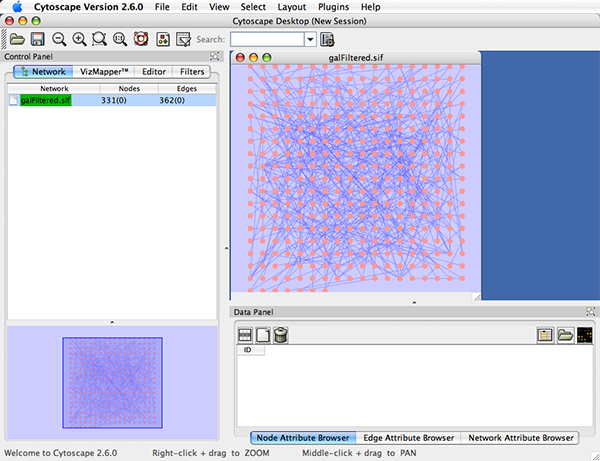
\includegraphics[width=\textwidth]{images/cytoscape_startup_network_26.png}
\caption{Cytoscape加载网络后的界面截图}
\label{fig:2.1}
\end{figure}

主界面由多个组件构成,包括:
\begin{itemize}
\item 顶部的菜单(稍后会对各个菜单做详细介绍)。
\item 工具栏,包含了各种常用功能。从菜单中也能使用这些功能。鼠标指针在这些图标上停留片刻就能看到有关的提示。
\item 网络管理面板(左上方的面板)。其中有可关闭的网络全局浏览面板(左下方)。
\item 网络查看主窗口,网络就显示在这个窗口中。
\item 属性浏览器面板(底部的面板),显示所选择的节点和边的属性。在这个面板中还可以对这些属性的值进行修改。
\end{itemize}

网络管理和属性浏览器面板是可以拖拽的标签面板,被称为~CytoPanels~。通过点击~CytoPanel~右上角的浮动窗口(Float Window)控件~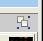
\includegraphics{images/float_icon.png}~可以将这些面板设为浮动状态。

如果选择了这个控件,例如属性浏览器面板上的这个控件,就会出现两个~Cytoscape~的窗口,一个是主窗口,另一个是名为CytoPanel 2的新窗口,如下图所示。当鼠标指针指向单元格时,会看到弹出信息。

{\centering
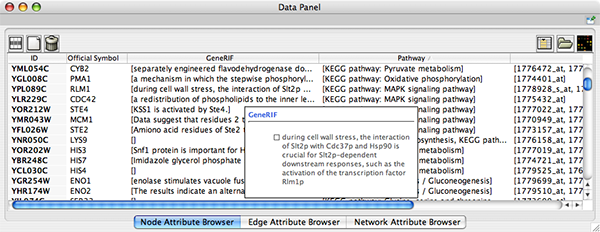
\includegraphics[width=\textwidth]{images/attribute_browser_26.png}
}

在图中可以看到,CytoPanel 2~现在有一个~Dock Window~控件。如果点选这个控件,这个窗口就会回到主窗口中。

Cytoscape~还提供了一个用于构建和编辑网络的编辑器,把面板中的节点和边拖拽到主网络视图窗口中就能创建和编辑网络。用Visual Style可以定义节点的形状以及边的箭头。只需要选择CytoPanel 1中的Editor标签就能编辑网络。下图展示了一个编辑器,Visual Style是BioMoleculeEditor。

{\centering
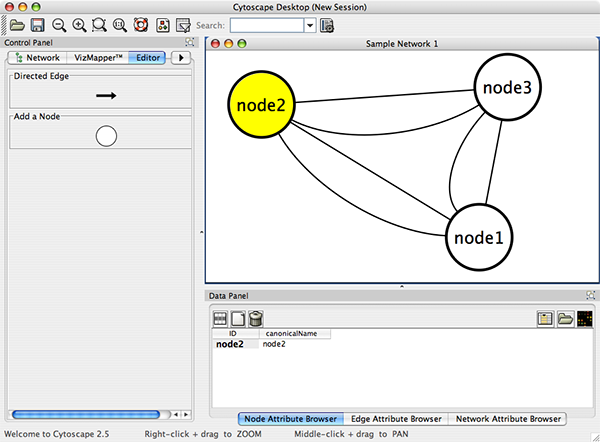
\includegraphics[width=\textwidth]{images/editor_25.png}}

\section{菜单}
	\subsection{File}
	File菜单中含有最基本的文件操作功能:File $\rightarrow$ Open~用于打开~Cytoscape~会话文件;File $\rightarrow$ New~用于新建空白网络,也可以从现用的网络创建新网络;File $\rightarrow$ Save~用于保存会话文件;File $\rightarrow$ Import~用于导入网络或属性数据;File $\rightarrow$ Export~用于导出数据和图片。File $\rightarrow$ Print用于打印,File $\rightarrow$ Quit~则是关闭所有的~Cytoscape~窗口,并推出程序。

	\centerline{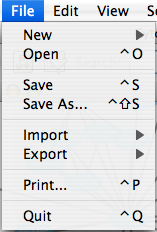
\includegraphics{images/menu_file_26.png} }

	\subsection{Edit}
	Edit菜单中提供了用于属性浏览器、网络编辑器和布局的撤销(Undo)和重做(Redo)功能。
	
	还有创建和销毁视图(网络的显示方法)和网络(网络的原始数据,并不可视化的)的菜单项,以及用于从当前网络中删除所选节点和边的菜单项。通过 Edit $\rightarrow$ Undo~可以恢复被删除的节点和边。配置和插件的设置可以通过Edit $\rightarrow$ Preferences $\rightarrow$ Properties来编辑。

	\centerline{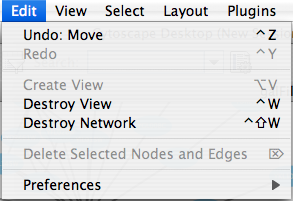
\includegraphics{images/menu_edit_26.png}}

	\subsection{View}
	在~View~菜单中可以控制网络管理面板(CytoPanel 1)、属性浏览器(CytoPanel 2)、网络概览(在CytoPanel 1中)和VizMapper的显示和隐藏。

	\centerline{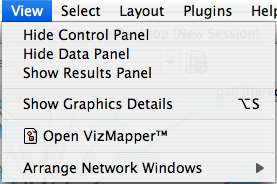
\includegraphics{images/menu_view_26.png}}

	\subsection{Select}
	在~Select~菜单中含有选择节点和边的各种选项。还有Select $\rightarrow$ Use Filter选项,用于根据节点或边的某些属性创建自动的过滤器。

	\centerline{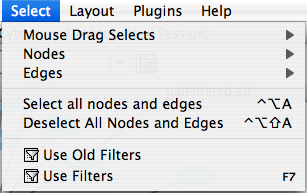
\includegraphics{images/menu_select_26.png}}

	\subsection{Layout}
		
	
	\subsection{Plugins}
	
	\subsection{Layout}
	
	\subsection{Help}

\section{网络管理}
	\subsection{网络窗口排列}

\section{网络概览窗口}
	




